%!TEX root = main.tex


\section{Variables and Probability Models}\label{sec:vague_variables}

\subsection{Why are variables functions?}\label{sec:variables}

Our theory is mainly concerned with \emph{Markov kernels}, which are functions that map from measurable sets to probability distributions. On their own, Markov kernels are just abstract mathematical objects, but we want to use them to make \emph{models} which aim to explain some part of the world. To make a Markov kernel into a model, we annotate it with a set of variables. The model relates variables to one another ``in the world of maths'', and the variables enable this to be interpreted as a claim about how some parts of the real world relate to one another.

As a simple example of a model, consider Newton's second law in the form $F=MA$, which relates variables $F$, $M$ and $A$. As \citet{feynman_feynman_1979} noted, this law is incomplete -- in order to understand it, we must bring some pre-existing understanding of force, mass and acceleration as independent things, not defined by this equation. As it happens, physicists know a great deal about determining the forces on an object. Nevertheless, in order to actually say what the force on an object is, even a highly knowledgeable physicist will still have to go and measure something.

This makes ``force'' $F$ and odd kind of object. It is not a well-defined mathematical thing, because it requires an action in the real world to determine its value, and such actions can not themselves be mathematically defined. At the same time, the set of values it takes is a well-defined mathematical thing. This is what enables an expression like ``$MA$'' to be sensibly interpreted --  $MA$ is itself a variable obtained by making a measurement of $M$ and $A$ and multiplies the resulting values. We will call objects like $F$, $M$ and $MA$ ``real-world variables''.

In general, if I have a variable $B$ that takes values in some set $X$, and a function $f:X\to Y$, call the composition $f\circ B$, itself a variable that takes values in $Y$, what I get by first measuring $B$ and then applying the function $f$ to the result.

In order to proceed, we assume we have a real-world variable that measures everything of interest and records it as some value. We can't understand the model $F=MA$ by providing a generic $F$ that measures some net force, $M$ that measures some mass and so forth. Rather, we require the mass, acceleration and forces on a particular object at a particular time, so we require $F,M$ and $A$ to all refer to the same object. In order to state this requirement, we have to talk about all three variables together. That is, a complete specification of the measurement to take place must detail how to measure $(F,M,A)$ all together. 

Our assumption is that a joint specification of every measurment of interest is available, and when conducted these measurements will yield a unique value in some well-defined set. This entire process is represented by the ``master'' real-world variable $S$. What we mean by the condition that $S$ contains every measurement of interest is, precisely, that any observed variable appearing in our model is obtained by composing a function with $S$ in the sense described above.

At this point, we have something that resembles the usual story: we can call the set of potential values of $S$ the ``sample space''. If we have some observed variable $X$ given by $f\circ S$, we can identify the ``random variable'' $\RV{X}:=f$.

Not every variable will be an observable variable. Unobserved and unobservable variables play a central role in causal inference. We suppose all such variables take values in well-defined sets, and that we can always propose values of unobserved variables.

To account for unobserved variables, we make the following rather inelegant assumption: there is some process $O$ that can take proposed values of unobserved variables, as well as make measurments of observed variables of interest, that returns values in some sample space $\Omega$. Values in $\Omega$ uniquely determine all quantities of interest in the sense that any variable $V$ taking values in $W$ that appears in our model is obtained by composing some function $\RV{V}:\Omega\to W$ with $O$; $V:=\RV{V}\circ O$ (where composition is defined as above: it is again a process that takes the output of $O$ and applies the function $\RV{V}$ to it).

Thus we confine all of the messy real-world interaction to this process $O$, and identify any variable $V$ with the function $\RV{V}$ we use to obtain $V$ from $O$. Before we sweep $O$ under the carpet completely, we want to note that we have placed some non-trivial requirements on it:

\begin{itemize}
	\item Given a proposed value of unobserved variables it must eventually produce a unique element of $\Omega$, once all measurements are complete
	\item For any variable $V$, we must be satisfied that $O$ followed by applying the function $\RV{V}$ to the output is indeed a measurement of the thing $V$ refers to
\end{itemize}

We don't make any presumptions about how $O$ and $\Omega$ are constructed, just that they can be. It may be possible to construct it in a fairly straightforward way -- for example, to do some set of measurments in arbitrary order, append all the values obtained and then append to them a set of proposed values of unobserved variables. On the other hand, perhaps some care is needed to specify how measurements can be done together and in what order. However it is accomplished, we just assume that it can be done.

Our basic setup is then: variables are \emph{defined} by the process $O$, and our \emph{models} are statements about how variables are probabilistically related to one another; $F=MA$ is an example of a model.

We consider two types of model: first, we consider models of the entire process $O$, which is analogous to the standard practice of starting off with a \emph{probability space}. We also consider partial models -- models that only relate a subset of variables to one another, and introduce the notion of \emph{compatibility} to indicate when such models are legitimate.

% For example, \citet{pearl_causality:_2009} offers the same definition of formal variables as we do, but also explains:
% \begin{quote}
% By a \emph{variable} we will mean an attribute, measurement or inquiry that may take on one of several possible outcomes, or values, from a specified domain. If we have beliefs (i.e., probabilities) attached to the possible values that a variable may attain, we will call that variable a random variable.
% \end{quote}

% We will call variables defined with reference to specific measurements \emph{observable variables}. How should we model variables of this kind? Suppose we have an observable variable $\RV{X}$ -- i.e. $\RV{X}$ represents an act of measurement (``the measurement of my height in centimetres I am about to perform'') and has a specified codomain (a natural number). Suppose we can consult $\RV{X}$ on multiple occasions -- say, first to write it in this paper (185cm) and secondly to discuss with my daughter later today. I cannot consult $\RV{X}$ before I measure my height, but once I have done so, in order for $\RV{X}$ to be well-defined, it must surely have the same value every time it is consulted.

% \citet{menger_random_2003}, under the name of \emph{qualitative statistical random variable}, offers the following definition of a variable that satisfies this condition. A qualitative statistical random variable is:
% \begin{itemize}
% 	\item A set of ordered pairs $(x,y)$, where $x$s are attributes, acts of measurement or inquiries and $y$s may take values in a specified codomain $Y$ 
% 	\item Each $x$ corresponds to exactly one $y$
% \end{itemize}

% Menger offers the examples of a variable that takes for $x$ people in Chicago and returns as $y$ their height in metres. The condition each $x$ corresponds to exactly one $y$ means that, if we go and do the experiment and measure the height of everybody in Chicago, each person will be assigned exactly one canonical height, and every time we query the height of a person $x$ we get the same height $y$.

% Our first condition for a model of observable variables is, if the value of an observable variable appears in multiple places, it must in all cases take the same value.

% Secondly, it is often useful to consider ``functions of variables''. For example, my daughter might want to know if she is more than half of my height. If my height is $\RV{X}$, then we will want to know what half my height is. We can consider this a second variable $\RV{H}$, whose codomain is multiples of $\frac{1}{2}$, with the property that whatever value $y$ is the ``actual'' value of $\RV{X}$, the value of $\RV{H}$ must be $\frac{y}{2}$. This induces a binary relation between the codomains of $\RV{X}$ and $\RV{H}$ consisting of the valid pairs of values $(y,\frac{y}{2})$.



% For theoretical tractability, however, we require formal definitions of observable variables. 
% \begin{align}
% 	\RV{X}=\RV{X}
% \end{align}

% An important question for our purposes is: when we define vague variables, what relationships should we understand them to have? This question can be illustrated with an example from the causal modelling framework of \emph{structural causal models}. This framework assigns a function to each variable. For example
% \begin{align}
% 	\RV{X}&=f_0(\xi_\RV{X})\label{eq:def_X}\\
% 	\RV{Y}&=f_1(\RV{X},\xi_{\RV{Y}})\label{eq:def_Y}
% \end{align}
% We may then \emph{intervene} on some or all variables. An intervention on $\RV{X}$, in this case, is an operation that generates a new set of structural equations identical to the previous set, except with the intervened variable having its equation modified in some manner (in this example, this could involve replacing Equation \ref{eq:def_X} with $\RV{X}=1$).

% Are the function assignments in a set of structural equations models of measurement processes? That is, if $\RV{X}$ is defined as a vague variable, is the function $\RV{X}\circ \xi_{\RV{X}}$ the model of the measurment process of interest? We think that the answer is \emph{no}. Interventions are typically meant to model actions that cause $\RV{X}$ to ``actually take on a different value'', not actions that alter the way we turn measurements into values. We could also say: if we intervene on $\RV{X}$, the way we determine the value of $\RV{X}$ from a measurement stays the same, but the result we get might be different. The \emph{definition of the variable} $\RV{X}$ is a higher-order commitment, which must be respected by any model of $\RV{X}$, while the definition of the \emph{structural equation associated with} $\RV{X}$ is a lower-order commitment which may be violated if we consider acting to change $\RV{X}$.

% Here we investigate an approach to probability modelling in which variables are higher-order commitments. That is, any valid model must satisfy constraints imposed by the definitions of variables. We show that this approach reduces to the standard approach under appropriate conditions, and is also a practical approach for dealing with the multiplicity of probability models that we often find ourselves considering when doing causal inference.

% This is a more difficult question when we expect to consider things that are not well-defined vague variables along with well-defined vague variables $\RV{X}$. 

% There are also other kinds of things we also use variables to model. For example, ``latent variables'' are by definition unobserved, so we cannot posit a story about them being defined by some ``process of observation''. Latent variables are often introduced in order to model relationships between observed variables, for example ``if the average height is $\RV{M}$ and the variance $\RV{V}$, then $\RV{X}_1$ will be distributed according to $\mathcal{N}(\RV{M},\RV{V})$''. We can extend the existential claim: there is some sample space and some collection of variables on it that describe the process of observing and supposing.

% However, for some questions we do need to be mindful of the complexities of vague variables, particularly when we are doing causal inference. Firstly, variables representing \emph{choices} may have a different scope to most types of variables. Consider two vague variables: $\RV{X}$ represents ``whether I get regular exercise next month'' and  $\RV{D}$ represents ``whether I decide to get regular exercise next month''. Many people might be able to observe my exercise next month, and therefore might be expected to agree on the value of $\RV{X}$ when all is said and done. On the other hand, most people won't be able to say what value $\RV{D}$ should take, as whether or not I contemplated a choice and what choice I took is information that will usually be available only to me. However, I will be able to say what value $\RV{D}$ took, and I will agree with my previous judgement if I ask myself this on multiple occasions.

% Secondly, the fact that a practical sample space might be constructible for a given set of vague variables does not imply that there is a practical way to consider the set of \emph{all} variables. Something like ``for every variable $\RV{Z}$, $\RV{Z}$ is not a common cause of $\RV{X}$ and $\RV{Y}$'' would seem to require consideration of all variables on the ``actual sample space'', whatever exactly that is, rather than a convenient summary.

\subsection{Probability, variables and composition}

Throughout this paper, we will assume all measurable sets are finite sets. This is because it makes explanations simpler and because it is easy to show that conditional probabilities exist in this setting (Lemma \ref{lem:subm_exist}).

We assume that there is some measurable sample space $\Omega$ and that all variables are measurable functions defined on $\Omega$. It is also often standard to assume that we have a \emph{probability space} $(\prob{P},(\Omega,\sigalg{F}))$, where $\prob{P}$ is a $\sigma$-additive measure on $(\Omega,\sigalg{F})$ with $\prob{P}(\Omega)=1$. Given such a probability space, the normal way to define the probability distribution of a particular random variable is via the \emph{pushforward measure}. Given $(\prob{P},(\Omega,\sigalg{F}))$ and $f_{\RV{X}}:(\Omega,\sigalg{F})\to (X,\sigalg{X})$, the pushforward measure is $\prob{P}^{\RV{X}} (A) := \prob{P}(\RV{X}^{-1}(A))$ for $A\in \sigalg{X}$.

We use a different approach to defining ``the distribution of $\RV{X}$''. Rather than defining it directly via the pushforward measure, we hold that, firstly, any contradictions by our definitions of random variables must be given probability 0, a property called \emph{consistency}, and secondly $\prob{P}^{\RV{X}}$ can be obtained from $\prob{P}^{\RV{XY}}$ by marginalising over $\RV{Y}$. Together with a probability $\prob{P}$ defined on the entire sample space, these recover the pushforward rule.

We will use the example of truncated factorisation to explain the motivation behind our approach. Consider ``truncated factorisation''. Suppose we have a causal Bayesian network $(\prob{P}^{\RV{XYZ}},\mathcal{G})$ where $\mathcal{G}$ is a Directed Acyclic Graph that contains the edges $\RV{X}\longrightarrowRHD \RV{Y}$ and $\RV{X}\longleftarrowRHD \RV{Z} \longrightarrowRHD \RV{Y}$. Then the result of ``setting $\RV{X}$ to $x$'' is represented by a new probability measure $\prob{P}_x$ that is required to obey truncated factorisation \citep[page ~24]{pearl_causality:_2009}:
\begin{align}
	\prob{P}^{\RV{XYZ}}_{x}(x',y,z)=\prob{P}^{\RV{Y|XZ}}(y|x,z)\prob{P}^{\RV{Z}}(z)\llbracket x=x' \rrbracket\label{eq:truncated_fac}
\end{align}

Equation \ref{eq:truncated_fac} embodies three assumptions. First, when we set $\RV{X}$ to $x$, then $\RV{X}\overset{a.s.}{=}x$. Second, when we set $\RV{X}$ to $x$, then $\RV{Z}$ carries on as before. Finally, $\RV{Y}$ given $\RV{X}$ and $\RV{Z}$ also carries on as before. These assumptions are not all equal in stature: the condition on the distribution of $\RV{X}$ is absolutely crucial: this is what it means to set $\RV{X}$ to $x$. The other two might be good assumptions if this causal Bayesian network happens to be good for our purposes.

However, there might be other assumptions that are more forceful than these latter two. For example, if $\RV{X}$ and $\RV{Z}$ happened to actually be the same random variables -- the same thing in the world that we go and look at -- then we absolutely must have $\RV{X}\overset{a.s.}{=}\RV{Z}$. The standard method for determining $\prob{P}^{\RV{XYZ}}_x$ will normally ensure that this condition is satisfied; that is, taking some $\prob{P}_x$ and compute the pushforward under $(\RV{X},\RV{Y},\RV{Z})$ will ensure $\RV{X}\overset{a.s.}{=}\RV{Z}$ if indeed $\RV{X}=\RV{Z}$.

However, $\RV{X}\overset{a.s.}{=}\RV{Z}$ cannot in general be satisfied at the same time as Equation \ref{eq:truncated_fac} for all $x$. Indeed, if $x$ may take more than one value, these two conditions cannot be simultaneously satisfied for at least one value of $x$.

So we have one critical assumption -- that $\RV{X}\overset{a.s.}{=}x$ -- from Equation \ref{eq:truncated_fac}, and another critical assumption -- that $\RV{X}\overset{a.s.}{=}\RV{Z}$ -- from the standard definition of what ``$\prob{P}^{\RV{XYZ}}_{x}$'' means, \emph{and} we know that Equation \ref{eq:truncated_fac} cannot actually be satisfied. This is obviously a mixed up situation. The condition of \emph{consistency}, which we introduce, addresses this problem. In this case, consistency demands $\RV{X}\overset{a.s.}{=}x$ and $\RV{X}\overset{a.s.}{=}\RV{Z}$ together, as we will show. Assumptions like Equation \ref{eq:truncated_fac} can be added as ``lower order'' demands of our probability model, but if they violate consistency then we must abandon them.

The assumption that $\RV{Z}=\RV{X}$ might seem forced, however we can consider a very similar situation if $\RV{Z}=(\RV{H},\RV{W})$, representing the height in metres and weight in kilograms of a particular person, and $\RV{X}$ represents their body mass index. In this case the causal structure we proposed is not original to us -- it appears in \citet{shahar_association_2009}. However, it is the case $\RV{X}=\frac{\RV{W}}{\RV{H}^2}$ and this also imposes a constraint that cannot be satisfied at the same time as \ref{eq:truncated_fac}.

The condition of consistency allows us to check when non-standard products like Equation \ref{eq:truncated_fac} yield ``well-formed'' probability models on the listed variables. We offer some sufficient conditions for probability models to be well-formed, which includes the case where the variables in question are surjective and \emph{variationally independent}, and if we have a strictly positive model over the same variables we already know to be well-formed.

We also show that the standard approach of defining a sample space model and defining marginals and conditionals via push-forwards is safe, in the sense that if the sample space model is well-formed then the marginals are well-formed and conditionals can always be chosen to be well-formed.

\subsection{Probability and composition without variables: Markov categories}
Markov categories are abstract categories that represent models of the flow of information. Operations like Equation \ref{eq:truncated_fac} are expressible as abstract compositions in Markov categories, and may be represented with string diagrams developed for reasoning about objects in the category. Valid proofs using string diagrams correspond to valid theorems in \emph{any} Markov category, though we will limit our attention to the category of finite sets and Markov kernels in this paper. The main drawback of Markov categories is that, as they exist at the moment, they have no notion of ``variables''. More comprehensive introductions to Markov categories can be found in \citet{fritz_synthetic_2020,cho_disintegration_2019}.

Rather than explain Markov categories in the abstract, we will introduce string diagrams with reference to how they represent stochastic maps and finite sets (though see Appendix \ref{sec:app_mcat}). Given measurable sets $(X,\sigalg{X})$ and $(Y,\sigalg{Y})$, a Markov kernel or stochastic map is a map $\kernel{K}:X\times \sigalg{Y}\to [0,1]$ such that

\begin{itemize}
	\item The map $x\mapsto \kernel{K}(x,A)$ is $\sigalg{X}$-measurable for every $A\in \sigalg{Y}$
	\item The map $A\mapsto \kernel{K}(x,A)$ is a probability measure for every $x\in X$
\end{itemize}

Where $X$ and $Y$ are finite sets with the discrete $\sigma$-algebra, we can represent a Markov kernel $\kernel{K}$ as a $|X|\times |Y|$ matrix where $\sum_{y\in Y} \kernel{K}_x^y = 1$ for every $x\in X$. We will give Markov kernels the signature $\kernel{K}:X\kto Y$ to indicate that they map from $X$ to probability distributions on $Y$.

Graphically, Markov kernels are drawn as boxes with input and output wires, and probability measures (which are kernels with the domain $\{*\}$) are represented by triangles:

\begin{align}
\kernel{K}&:=\begin{tikzpicture}[baseline={([yshift=-.5ex]current bounding box.center)}]
	\path (0,0) node (A) {}
	++ (0.5,0) node[kernel] (K) {$\kernel{K}$}
	++ (0.5,0) node (B) {};
	\draw (A) -- (K) -- (B);
\end{tikzpicture}\\
\kernel{P}&:= \begin{tikzpicture}[baseline={([yshift=-.5ex]current bounding box.center)}]
	\path (0,0) node[dist] (K) {$\kernel{P}$}
	++ (0.5,0) node (B) {};
	\draw (K) -- (B);
\end{tikzpicture}
\end{align}

Two Markov kernels $\kernel{L}:X\kto Y$ and $\kernel{M}:Y\kto Z$ have a product $\kernel{L}\kernel{M}:X\kto Z$ given by the matrix product $\kernel{L}\kernel{M}_x^z = \sum_y \kernel{L}_x^y\kernel{M}_y^z$. Graphically, we write represent by joining wires together:

\begin{align}
	\kernel{L}\kernel{M}:= \begin{tikzpicture}[baseline={([yshift=-.5ex]current bounding box.center)}]
	\path (0,0) node (A) {}
	++ (0.5,0) node[kernel] (K) {$\kernel{K}$}
	++ (0.7,0) node[kernel] (M) {$\kernel{M}$}
	++ (0.5,0) node (B) {};
	\draw (A) -- (K) -- (M) -- (B);
\end{tikzpicture}
\end{align}

The Cartesian product $X\times Y:=\{(x,y)|x\in X, y\in Y\}$. Given kernels $\kernel{K}:W\kto Y$ and $\kernel{L}:X\kto Z$, the tensor product $\kernel{K}\otimes\kernel{L}:W\times X\kto Y\times Z$ is defined by $(\kernel{K}\otimes\kernel{L})_{(w,x)}^{(y,z)}:=K_{w}^y L_{x}^z$ and represents applying the kernels in parallel to their inputs.

The tensor product is represeted by drawing kernels in parallel:

\begin{align}
	\kernel{K}\otimes \kernel{L}&:=\begin{tikzpicture}[baseline={([yshift=-.5ex]current bounding box.center)}]
	\path (0,0) node (A) {$W$}
	++ (0.5,0) node[kernel] (K) {$\kernel{K}$}
	++ (0.5,0) node (B) {$Y$};
	\path (0,-0.5) node (C) {$X$}
	++ (0.5,0) node[kernel] (L) {$\kernel{L}$}
	++ (0.5,0) node (D) {$Z$};
	\draw (A) -- (K) -- (B);
	\draw (C) -- (L) -- (D);
\end{tikzpicture}
\end{align}

We read diagrams from left to right (this is somewhat different to \citet{fritz_synthetic_2020,cho_disintegration_2019,fong_causal_2013} but in line with \citet{selinger_survey_2010}). A diagram describes products and tensor products of Markov kernels, which are expressed according to the conventions described above. There are a collection of special Markov kernels for which we can replace the generic ``box'' of a Markov kernel with a diagrammatic elements that are visually suggestive of what these kernels accomplish.

A description of these kernels follows.

The identity map $\text{id}_X:X\kto X$ defined by $(\text{id}_X)_x^{x'}= \llbracket x = x' \rrbracket$, where the iverson bracket $\llbracket \cdot \rrbracket$ evaluates to $1$ if $\cdot$ is true and $0$ otherwise, is a bare line:

\begin{align}
	\mathrm{id}_X&:=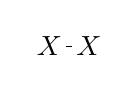
\begin{tikzpicture}[baseline={([yshift=-.5ex]current bounding box.center)}]
	\path (0,0) node (A) {$X$} ++ (0.5,0) node (B) {$X$};
	\draw (A) -- (B);
\end{tikzpicture}
\end{align}

We choose a particular 1-element set $\{*\}$ that acts as the identity in the sense that $\{*\}\times A=A\times \{*\} = A$ for any set $A$. The erase map $\text{del}_X:X\kto \{*\}$ defined by $(\text{del}_X)_x^* = 1$ is a Markov kernel that ``discards the input'' (we will later use it for marginalising joint distributions). It is drawn as a fuse:

\begin{align}
	\text{del}_X&:=\begin{tikzpicture}[baseline={([yshift=-.5ex]current bounding box.center)}]
	\path (0,0) ++ (1,0) node (B) {$X$};
	\draw[-{Rays[n=8]}] (A) -- (B);
\end{tikzpicture}
\end{align}

The copy map $\text{copy}_X:X\kto X\times X$ defined by $(\text{copy}_X)_x^{x',x''}=\llbracket x=x' \rrbracket \llbracket x=x'' \rrbracket$ is a Markov kernel that makes two identical copies of the input. It is drawn as a fork:

\begin{align}
	\text{copy}_X&:=\begin{tikzpicture}[baseline={([yshift=-.5ex]current bounding box.center)}]
	\path (0,0) node (A) {$X$} 
	++ (0.5,0) node[copymap] (copy0) {}
	++ (0.5,0.15) node (B) {$X$}
	+ (0,-0.3) node (C) {$X$};
	\draw (A) -- (copy0) to [out=45,in=180] (B) (copy0) to [out=-45, in=180] (C);
\end{tikzpicture}
\end{align}

The swap map $\text{swap}_{X,Y}:X\times Y\kto Y\times X$ defined by $(\text{swap}_{X,Y})_{x,y}^{y',x'}=\llbracket x=x' \rrbracket\llbracket y=y' \rrbracket$ swaps two inputs, and is represented by crossing wires:

\begin{align}
	\text{swap}_X &:=  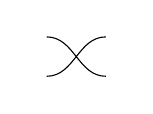
\begin{tikzpicture}[baseline={([yshift=-.5ex]current bounding box.center)}]
		\path (0,0) node (A) {} 
		+ (0,-0.5) node (B) {}
		++ (1,0) node (C) {}
		+ (0,-0.5) node (D) {};
		\draw (A) to [out=0,in=180] (D) (B) to [out=0, in=180] (C);
	\end{tikzpicture}
\end{align}

Because we anticipate that the graphical notation will be unfamiliar to many, we will also include translations to more familiar notation.

\subsection{Truncated factorisation with Markov kernels}

The Markov kernels introduced in the previous section can be though of as ``conditional probability distributions without variables''. We can use these to represent an operation very similar to Equation \ref{eq:truncated_fac}. Note that $P^{\RV{Y|XZ}}$ must be represented by a Markov kernel $\kernel{K}:X\times Z\kto Y$ and $\prob{P}^{\RV{Z}}$ by a Markov kernel $\kernel{L}\in \Delta(Z)$. Then we can define a Markov kernel $\kernel{M}:X\kto X\times Z$ representing $x\mapsto \prob{P}^{\RV{YZ}}_{x}(y,z)$ by

\begin{align}
	\kernel{M}:= \tikzfig{truncated_factorisation}\label{eq:tfac_setted}
\end{align}

There is, however, a key difference between Equation \ref{eq:tfac_setted} and Equation \ref{eq:truncated_fac}: the Markov kernels in the latter equation describe the distribution of particular variables, while the former equation describes Markov kernels only.

To illustrate why we need variables, consider an arbitrary Markov kernel $\kernel{K}:\{*\}\kto \Delta(X\times X)$. We could draw this:
\begin{align}
	\kernel{K}:= \tikzfig{double_label}\label{eq:double_label}
\end{align}
We label both wires with the set $X$. However, say $X=\{0,1\}$. Then $\kernel{K}$ could be the kernel $\kernel{K}^{x_1,x_2} = \llbracket x_1 = 0\rrbracket \llbracket x_2 = 1\rrbracket$. In this case, both of its outputs must represent \emph{different} variables, despite taking values in the same set. On the other hand, if $\kernel{K}^{x_1,x_2} = 0.5 \llbracket x_1 = x_2 \rrbracket$ then both outputs coudl represent the same variable, because they are deterministically the same, or they could represent different variables that happen to be equal. We need some way to distinguish the two cases.


\subsection{Composition and probability with variables}

Our goal is to define a category of ``finite sets and Markov kernels with variables''. Introducing variables requires an assumption of consistency, which we don't know how to express in category theoretic terms. Our approach is to define a category of Markov kernels with variables that may or may not be consistent, which we will need to check for the resulting models. Because the consistency assumption is not expressed category theoretically, many proofs in this section only apply to our chosen setting of finite sets.

\begin{definition}[Variable]
Given a \emph{sample space} $\Omega$, a variable $f_\RV{X}$ is a function $\Omega\to A$ where $A$ is a vector space. We will also refer to the associated Markov kernel $\RV{X}:\Omega\kto A$
as a variable, where $\RV{X}_x^a=\llbracket a = f_{\RV{X}}(x) \rrbracket$.
\end{definition}

We define the \emph{product} of two variables as follows:
\begin{itemize}
	\item \textbf{Product:} Given variables $\RV{W}:\Omega\kto A$ and $\RV{V}:\Omega\kto B$, the product is defined as $(\RV{W}, \RV{V})=\text{copy}_{\Omega} (\RV{W}\otimes\RV{V})$
\end{itemize}

The \emph{unit} variable is the erase map $\RV{I}:=\text{del}_\Omega$, with $(\RV{I},\RV{X})=(\RV{X},\RV{I})=\RV{X}$ (up to isomorphism) for any $\RV{X}$.

We then need a notion of Markov kernels that ``maps between variables''. An \emph{indexed Markov kernel} is such a thing.

\begin{definition}[Indexed Markov kernel]
Given variables $\RV{X}:\Omega\to A$ and $\RV{Y}:\Omega\to B$, an indexed Markov kernel $\kernel{K}:\RV{X}\kto \RV{Y}$ is a triple $(\kernel{K}',\RV{X},\RV{Y})$ where $\kernel{K}':A\kto B$ is the \emph{underlying kernel}, $\RV{X}$ is the \emph{input index} and $\RV{Y}$ is the \emph{output index}.
\end{definition}

For example, if $\kernel{K}:(\RV{A}_1,\RV{A}_2)\to \Delta(\RV{B}_1,\RV{B}_2)$, for example, we can draw:

\begin{align}
	\kernel{K} := \begin{tikzpicture}[baseline={([yshift=-.5ex]current bounding box.center)}]
	\path (0,0) node (A1) {$\RV{A}_1$}
	+ (0,-0.3) node (A2) {$\RV{A}_2$}
	++ (0.7,-0.15) node[kernel] (K) {$\kernel{K}$}
	++ (0.7,0.15) node (B1) {$\RV{B}_1$}
	+ (0,-0.3) node (B2) {$\RV{B}_2$};
	\draw (A1) -- ($(K.west) + (0,0.15)$) (A2) -- ($(K.west) + (0,-0.15)$);
	\draw (B1) -- ($(K.east) + (0,0.15)$) (B2) -- ($(K.east) + (0,-0.15)$);
\end{tikzpicture}
\end{align}

or

\begin{align}
	\kernel{K} = \begin{tikzpicture}[baseline={([yshift=-.5ex]current bounding box.center)}]
	\path (0,0) node (A1) {$(\RV{A}_1,\RV{A}_2)$}
	++ (1.3,0) node[kernel] (K) {$\kernel{K}[\model{L}]$}
	++ (1.3,0.) node (B1) {$(\RV{B}_1,\RV{B}_2)$};
	\draw (A1) -- (K) -- (B1);
\end{tikzpicture}
\end{align}

We define the product of indexed Markov kenrnels $\kernel{K}:\RV{X}\kto \RV{Y}$ and $\kernel{L}:\RV{Y}\kto \RV{Z}$ as the triple $\kernel{K}\kernel{L}:=(\kernel{K}'\kernel{L}',\RV{X},\RV{Z})$.

Similarly, the tensor product of $\kernel{K}:\RV{X}\kto\RV{Y}$ and $\kernel{L}:\RV{W}\kto\RV{Z}$ is the triple $\kernel{K}\otimes\kernel{L}:=(\kernel{K}'\otimes\kernel{L}',(\RV{X},\RV{W}),(\RV{Y},\RV{Z}))$.

We define $\text{Id}_{\RV{X}}$ to be the model $(\text{Id}_X,\RV{X},\RV{X})$, and similarly the indexed versions $\text{del}_{\RV{X}}$, $\text{copy}_{\RV{X}}$ and $\text{swap}_{\RV{X},\RV{Y}}$ are obtained by taking the unindexed versions of these maps and attaching the appropriate random variables as indices. Diagrams are the diagrams associated with the underlying kernel, with input and output wires annotated with input and output indices.

The category of indexed Markov kernels as morphisms and variables as objects is a Markov category (Appendix \ref{sec:app_mcat}), and so a valid derivation based on the string diagram language for Markov categories corresponds to a valid theorem in this category. However, most of the diagrams we can form are not viable candidates for models of our variables. For example, if $\RV{X}$ takes values in $\{0,1\}$ we can propose an indexed Markov kernel $\kernel{K}:\RV{X}\kto\RV{X}$ with $\kernel{K}_a^{\prime b}=0.5$ for all $a, b$. However, this is not a useful model of the variable $\RV{X}$ -- it expresses something like ``if we know the value of $\RV{X}$, then we belive that $\RV{X}$ could take any value with equal probability''.

We define a \emph{model} as ``an indexed Markov kernel that assigns probability 0 to things known to be contradictions''. A contradiction is a simultaneous assignment of values to the variables $\RV{X}$ and $\RV{Y}$ such that there is no value of $\omega$ under which they jointly take these values. Unless the value assignment to the domain variable is itself contradictory, we hold that any valid model must assign probability zero to such occurrences.

\begin{definition}[Probabilistic model]
An indexed Markov kernel $(\kernel{K}',\RV{X},\RV{Y})$ is a \emph{probabilistic model} (``model'' for short) if it is \emph{consistent}, which means it assigns probability 0 to contradictions:
\begin{align}
	f_{\RV{X}}^{-1}(a)\cap f_{\RV{Y}}^{-1}(b) = \emptyset \implies \left(\kernel{K}_{a}^{\prime b} = 0\right) \lor \left(f_{\RV{X}}^{-1}(a) = \emptyset\right)
\end{align}
A \emph{probability model} is a model where the underlying kernel $\kernel{K}'$ has the unit $\RV{I}$ as the domain. We use the font $\model{K}$ to distinguish models from arbitrary indexed Markov kernels.
\end{definition}

Consistency implies that for any $\model{K}:\RV{X}\kto\RV{Y}$, if $f_{\RV{Y}}=g\circ f_{\RV{X}}$ then $\model{K}_x^{g(x)}=1$. A particularly simple case of this is a model $\model{L}:\RV{X}\kto\RV{X}$, which must be such that $\model{L}_x^x=1$. \citet{hajek_what_2003} has pointed out that standard definitions of conditional probability allow the conditional probability to be arbitrary on a set of measure zero, even though ``the probability $\RV{X}=x$, given $\RV{X}=x$'' should obviously be 1.

We take the idea of marginal distributions as fundamental.

\begin{definition}[Marginal distribution]
Given a model $\model{K}:\RV{X}\kto(\RV{Y},\RV{Z})$, the marginal distribution of $\RV{Y}$, written $\model{K}^{\RV{Y}|\RV{X}}$, is obtained by marginalising over $\RV{Z}$:
\begin{align}
	\model{K}^{\RV{Y}|\RV{X}} &:= \tikzfig{marginal}\\
	&\iff\\
	(\model{K}^{\RV{Y}|\RV{X}})_x^y &= \sum_{z\in Z} \kernel{K}_x^{\prime yz}
\end{align}
\end{definition}

\begin{definition}[Disintegration]
Given a model $\model{K}:\RV{X}\kto(\RV{Y},\RV{Z})$, a disintegration $\model{L}:(\RV{X},\RV{Y})\kto \RV{Z}$ $\RV{Y}$, written $\model{K}^{\RV{Y}|\RV{X}}$, is obtained by marginalising over $\RV{Z}$
\end{definition}

We can always get a valid model by adding a copy map to a valid model, and conversely all valid models with repeated codomain variables must contain copy maps.

\begin{lemma}[Output copies of the same variable are identical]\label{lem:nocopy1}
For any $\kernel{K}:\RV{X}\kto (\RV{Y},\RV{Y},\RV{Z})$, $\kernel{K}$ is a model iff there exists some $\model{L}:\RV{X}\kto (\RV{Y},\RV{Z})$ such that
\begin{align}
		\kernel{K} &= \tikzfig{compose_with_copymap}\\
		&\iff \\
		\kernel{K}_{x}^{\prime y,y',z} &= \llbracket y=y' \rrbracket\kernel{L}_{x}^{\prime y,z}\\
\end{align}
\end{lemma}


\begin{proof}
$\implies$
For any $\omega,x,y,y',z$:
\begin{align}
	(\RV{X},\RV{Y},\RV{Y},\RV{Z})_\omega^{x,y,y',z} &= \llbracket f_{\RV{Y}}(\omega)=y \rrbracket \llbracket f_{\RV{Y}}(\omega)=y' \rrbracket (\RV{X},\RV{Z})_\omega^{x,z} \\
	&= \llbracket y=y' \rrbracket \llbracket f_{\RV{Y}}(\omega)=y \rrbracket(\RV{X},\RV{Z})_\omega^{x,z}
\end{align}
Therefore, by consistency, for any $x,y,y',z$, $y\neq y'\implies \kernel{K}_{x}^{\prime yy'z}=0$. Define $\kernel{L}$ by $\kernel{L}_x^{\prime y, z} := \kernel{K}_x^{\prime y y z}$. The fact that $\model{L}$ is a model follows from the assumption that $\model{K}$ is. Then
\begin{align}
	\kernel{K}_{x}^{\prime y,y',z} &= \llbracket y=y' \rrbracket\kernel{L}_{x}^{\prime y,z}
\end{align}
$\Leftarrow$
If $\model{L}$ is a model, then for any $x,x',y,z$, 
\begin{align}
\llbracket y=y'\rrbracket \model{L}_{x}^{\prime y,z}>0&\implies y=y'\land \model{L}_{x}^{\prime y,z}>0\\
													  &\implies \left(f_{\RV{X}}^{-1}(x)=\emptyset \right)\lor \left(f_{\RV{X}}^{-1}(x)\cap f_{\RV{Y}}^{-1}(y) \cap f_{\RV{Y}}^{-1}(y)\cap f_{\RV{Z}}^{-1}(z)\neq\emptyset \right)\\
\end{align}
\end{proof}

We can always get a valid model by copying the input to the output of a valid model, and conversely all valid models where there is a variable shared between the input and the output must copy that input to the output.

\begin{lemma}[Copies shared between input and output are identical]\label{lem:nocopy2}
For any $\kernel{K}:(\RV{X},\RV{Y})\kto (\RV{X},\RV{Z})$, $\kernel{K}$ is a model iff there exists some $\model{L}:(\RV{X},\RV{Y})\kto \RV{Z}$ such that
\begin{align}
	 \kernel{K} &= \tikzfig{precompose_with_copymap}\\
	 &\iff\\
	 \kernel{K}_{x,y}^{\prime x',z} &= \llbracket x=x'\rrbracket \kernel{L}_{\prime x,y}^{z}
\end{align}
\end{lemma}

\begin{proof}
$\implies$
For any $\omega,x,y,y',z$:
\begin{align}
	(\RV{X},\RV{Y},\RV{Y},\RV{Z})_\omega^{x,y,y',z} &= \llbracket f_{\RV{Y}}(\omega)=y \rrbracket \llbracket f_{\RV{Y}}(\omega)=y' \rrbracket (\RV{X},\RV{Z})_\omega^{x,z} \\
	&= \llbracket y=y' \rrbracket \llbracket f_{\RV{Y}}(\omega)=y \rrbracket(\RV{X},\RV{Z})_\omega^{x,z}
\end{align}
Therefore, by consistency, for any $x,y,y',z$, $x\neq x'\implies \model{K}_{x,y}^{\prime x'z}=0$. Define $\kernel{L}$ by $\kernel{L}_{x,y}^{\prime x', z} := \model{K}_{x,y}^{\prime x, y}$. The fact that $\kernel{L}$ is a model follows from the assumption that $\model{K}$ is a model. Then
\begin{align}
	\kernel{K}_{x, y}^{\prime x', z} &= \llbracket x=x' \rrbracket\kernel{L}_{x,y}^{\prime z}
\end{align}
$\Leftarrow$
If $\model{L}$ is a model, then for any $x,x',y,z$, 
\begin{align}
\llbracket x=x'\rrbracket \model{L}_{ x,y}^{\prime z}>0&\implies x=x'\land \model{L}_{ x,y}^{\prime z}>0\\
													  &\implies \left( f_{\RV{X}}^{-1}(x)\cap f_{\RV{Y}}^{-1}(y)=\emptyset \right)\lor \left(f_{\RV{X}}^{-1}(x)\cap f_{\RV{X}}^{-1}(x)\cap f_{\RV{Y}}^{-1}(y)\cap f_{\RV{Z}}^{-1}(z)\neq\emptyset \right)\\
\end{align}
\end{proof}

Consistency along with the notion of marginal distributions implies that, given some $\RV{X}$ and some $\model{K}:\RV{Y}\kto\text{Id}_\Omega$, the pushforward $\model{K}\model{X}$ is the unique model $\RV{Y}\kto \RV{X}$ that can be paired (Definition \ref{def:pairing}) with $\model{K}$. This is shown in Lemma \ref{lem:pushforward}.

\begin{lemma}[Uniqueness of models with the sample space as a domain]\label{lem:uniq_model}
For any $\RV{X}:\Omega\to A$, there is a unique model $\model{X}:\text{Id}_\Omega\kto \RV{X}$ given by $\model{X}:=(\RV{X},\text{Id}_\Omega,\RV{X})$.
\end{lemma}

\begin{proof}
$\RV{X}$ is a Markov kernel mapping from $\Omega\to A$, so it is a valid underlying kernel for $\model{X}$, and $\model{X}$ has input and output indices matching its signature. We need to show it satisfies consistency.

For any $\omega\in \Omega$, $a\in A$
\begin{align}
	\max_{\omega\in \Omega}(\text{Id}_\Omega,\RV{X})_{\omega}^{\omega',a} &= \max_{\omega\in \Omega} \llbracket \omega = \omega' \rrbracket \llbracket \omega = f_{\RV{X}}(a) \rrbracket\\
	&= \llbracket \omega = f_{\RV{X}}(a) \rrbracket\\
	&= \kernel{X}_\omega^a
\end{align}
Thus $\model{X}$ satisfies consistency.

Suppose there were some $\model{K}:\text{Id}_\Omega\kto \RV{X}$ not equal to $\RV{X}$. Then there must be some $\omega\in \Omega$, $b\in A$ such that $\model{K}_\omega^b\neq 0$ and $f_{\RV{X}}(\omega)\neq b$. Then
\begin{align}
	\max_{\omega\in \Omega}(\text{Id}_\Omega,\RV{X})_{\omega}^{\omega',a} &= \max_{\omega\in \Omega} \llbracket \omega = \omega' \rrbracket \llbracket \omega = f_{\RV{X}}(b) \rrbracket\\
	&= \llbracket \omega = f_{\RV{X}}(b) \rrbracket\\
	&= 0\\
	&< \model{K}_\omega^b
\end{align}
Thus $\model{K}$ doesn't satisfy consistency.
\end{proof}

% \begin{corollary}[Uniqueness of joint models]\label{cor:uniq_joint}
% For any $\RV{X}:\Omega\to A$, there is a unique model $\model{X}:\text{Id}_\Omega\kto (\RV{X},\text{Id}_{\Omega})$.
% \end{corollary}

% \begin{proof}
% Apply Lemma \ref{lem:nocopy2} to the model $\model{X}$ from Lemma \ref{lem:uniq_model}.
% \end{proof}

\begin{definition}[Pairing]\label{def:pairing}
Two models $\model{K}:\RV{X}\kto \RV{Y}$ and $\model{L}:\RV{X}\kto \RV{Z}$ can be \emph{paired} if there is some $\model{M}:\RV{X}\kto (\RV{Y},\RV{Z})$ such that $\model{K}=\model{M}^{\RV{Y}|\RV{X}}$ and $\model{L}=\model{M}^{\RV{Z}|\RV{X}}$.
\end{definition}

\begin{lemma}[Pushforward model]\label{lem:pushforward}
Given any model $\model{K}:\RV{Y}\kto \text{Id}_\Omega$ and any $\RV{X}$, there is a unique $\model{L}:\RV{Y}\kto \RV{X}$ that can be paired with $\model{K}$, and it is given by $(\kernel{L}^a_b = \sum_{\omega\in f_{\RV{X}}^{-1}(a)} \kernel{K}_b^{\omega}$.
\end{lemma}

\begin{proof}
Suppose that there is some $\model{L}$ that can be paired with $\model{K}$ via some $\model{M}:\RV{Y}\kto(\text{Id}_\Omega,\RV{X})$. Then, by the existence of disintegrations, there must be some $\model{N}:\text{Id}_{\Omega}\kto \RV{X}$ such that
\begin{align}
	\model{M}&=\tikzfig{disintegration_omega}
\end{align}
By Corollary \ref{cor:uniq_joint}, there is only one model $\model{N}:\text{Id}_{\Omega}\kto \RV{X}$ is unique and equal to $\model{X}:=(\RV{X},\text{Id}_\Omega,\RV{X})$.

It remains to be shown that $\model{M}$ is also a model. We already know that $\model{K}$ is consistent with respect to $(\RV{Y},\text{Id}_\Omega)$ and $\model{L}$ is consistent with respect to $(\text{Id}_\Omega,\RV{X})$. $\model{M}$ must be consistent with respect to $(\RV{Y},\text{Id}_\Omega,\RV{X})$. Consider any $x\in X$, $\omega\in \Omega$, $y\in Y$ such that $f_{\RV{X}}^{-1}(x)\cap \{\omega\}\neq \emptyset$ and $f_{\RV{Y}}^{-1}(y)\cap\{\omega\}\neq \emptyset$. Trouble might arise if $f_{\RV{X}}^{-1}(x)\cap \{\omega\} \cap f_{\RV{Y}}^{-1}(y)=\emptyset$, but this is obviously impossible as $\omega\in f_{\RV{X}}^{-1}(x)$ and $\omega\in f_{\RV{Y}}^{-1}(y)$.

Finally, for any $a\in A$, $b\in B$
\begin{align}
	(\model{K}\model{X})^a_b &= \sum_{\omega\in \Omega} \model{P}_b^\omega\RV{X}_\omega^a\\
						 &= \sum_{\omega\in \Omega} \model{P}_b^\omega \llbracket a = f_{\RV{X}}(\omega) \rrbracket\\
						 &= \sum_{\omega\in f^{-1}(a)} \model{P}_b^{\omega}
\end{align}
\end{proof}

\begin{corollary}[Pushforward probability model]\label{corr:pushforward}
Given any probability model $\model{P}:\RV{I}\kto \text{Id}_\Omega$, there is a unique model $\model{P}^{\RV{X}}:\RV{I}\kto \RV{X}$ such that $\model{P}^{\RV{X}}=\model{P}\model{Q}$ for some $\model{Q}:\text{Id}_\Omega\to \RV{X}$, and it is given by $(\model{P}^{\RV{X}})^a_b = \sum_{\omega\in f^{-1}(a)} \model{P}_b^{\omega}$.
\end{corollary}

\begin{proof}
Apply Lemma \ref{lem:pushforward} to a model $\model{P}:\RV{I}\kto\text{Id}_{\Omega}$.
\end{proof}

The following lemmas can help us check whether an indexed Markov kernel is a valid model.



We take the following term from \citet{constantinou_extended_2017}. Our definition is equivalent to unconditional variation independence in that paper.

\begin{definition}[Variation independence]
Two variables $\RV{X}:\Omega\kto X$ and $\RV{Y}:\Omega\kto Y$ are variation independent, written $\RV{X}\perp_v \RV{Y}$, if for all $y\in f_\RV{Y}(\Omega)R(f_{\RV{Y}})$
\begin{align}
 f_\RV{Y}(\Omega) \times f_{\RV{X}}(\Omega) = \{(f_{\RV{Y}}(\omega),f_{\RV{X}}(\omega))|\omega\in \Omega\}
\end{align}
\end{definition}

If a collection of variables is variation independent and surjective, then an arbitrary indexed Markov kernel labelled with these variables is a model.

\begin{lemma}[Consistency via variation conditional independence]\label{lem:var_indep}
Given an indexed Markov kernel $\kernel{K}:\RV{X} \kto \RV{Y}$ with $\RV{X}:\Omega\kto X$ and $\RV{Y}:\Omega\kto Y$, if $f_\RV{Y}$ is surjective and $\RV{Y}\perp_v \RV{X}$ then $\kernel{K}$ is a model.
\end{lemma}

\begin{proof}
By variation independence and surjectivity of $f_{\RV{Y}}$, for any $x\in X$, $y\in Y$, $f_{\RV{X}}^{-1}(x)\cap f_{\RV{Y}}^{-1}(y) = \emptyset \implies f_{\RV{X}}^{-1}(x) = \emptyset$. Thus the criterion of consistency places no restrictions on $\kernel{K}$.
\end{proof}

\todo[inline]{I think Lemmas \ref{lem:nocopy1} and \ref{lem:nocopy2} might be sufficient to offer diagrammatic checks of consistency if all variables that are not identical are variation independent. This is probably an interesting result, but I'm not sure if it's a higher priority than filling out the rest of the content.}

Alternatively, if we have a strictly positive indexed Markov kernel that is known to be a model, we can conclude that arbitrary indexed Markov kernels with appropriate labels are also models.

\begin{lemma}[Consistency via positive models]\label{lem:avoid_contradic}
Given a model $\model{K}:\RV{X}\kto (\RV{Y},\RV{Z})$, if an indexed Markov kernel $\kernel{L}:(\RV{X},\RV{Y})\kto \RV{Z}$ has the property $\kernel{K}_x^{\prime yz}=0\implies \kernel{L}_{xy}^{\prime z}=0$ then $\kernel{L}$ is also a model.
\end{lemma}

\begin{proof}
Because $\model{K}$ is a model,
\begin{align}
	\kernel{L}_{xy}^{\prime z}>0 &\implies \kernel{K}_x^{\prime yz} >0 \\
	&\implies \left( f_\RV{X}^{-1}(x)\cap f_\RV{Y}^{-1}(y)\cap f_\RV{Z}^{-1}(z) \neq \emptyset \right) \lor \left(f_\RV{X}^{-1}(x) = \emptyset \right)\\
	&\implies \left( f_\RV{X}^{-1}(x)\cap f_\RV{Y}^{-1}(y)\cap f_\RV{Z}^{-1}(z) \neq \emptyset \right) \lor \left(f_\RV{X}^{-1}(x)\cap f_{\RV{Y}}^{-1}(y) = \emptyset \right)
\end{align}
\end{proof}

\subsection{Truncated factorisation with variables}

At this point, we can represent Equation \ref{eq:truncated_fac} using models. Suppose $P^{\RV{Y|XZ}}$ is an model $\model{K}:(\RV{X}, \RV{Z})\kto \RV{Y}$ and $\prob{P}^{\RV{Z}}$ an model $\model{L}:\{*\}\kto \RV{Z}$. Then we can define an indexed Markov kernel $\kernel{M}:\RV{X}\kto \RV{X}, \RV{Z}$ representing $x\mapsto \prob{P}^{\RV{YZ}}_{x}(y,z)$ by

\begin{align}
	\kernel{M}&:= \tikzfig{truncated_factorisation_labeled}\label{eq:tfac_labeled}
\end{align}

Equation \ref{eq:tfac_labeled} is almost identical to Equation \ref{eq:tfac_setted}, except it now specifies which variables each measure applies to, not just which sets they take values in. Like the original Equation \ref{eq:truncated_fac}, there is no guarantee that $\kernel{M}$ is actually a model. If $f_\RV{X}=g\circ f_\RV{Z}$ for some $g:Z\to X$ and $X$ has more than 1 element, then the rule of consistency will rule out the existence of any such model.

If we want to use $\kernel{M}$, we want it at minimum to satisfy the consistency condition. One approach we could use is to check the result using Lemmas \ref{lem:nocopy1} to \ref{lem:avoid_contradic}, although note that \ref{lem:var_indep} and \ref{lem:avoid_contradic} are sufficient conditions, not necessary ones.

\subsection{Sample space models and submodels}

Instead of trying to assemble probability models as in Equation \ref{eq:tfac_labeled}, we might try to build probability models in a manner closer to the standard setup -- that is, we start with a sample space model (or a collection of sample space models) and work with marginal and conditional probabilities derived from these, without using any non-standard model assemblies.

A sample space model is any model $\kernel{K}:\RV{X}\kto \text{Id}_\Omega$. We expect that the collection of models under consideration will usually be defined on some small collection of random variables, but every such model is the pushforward of some sample space model. Using sample space models allows us to stay close to the usual convention of probability modelling that starts with a sample space probability model.

\begin{lemma}[Existence of sample space model]\label{lem:ss_exist}
Given any model $\model{K}:\RV{X}\kto \RV{Y}$, there is a sample space model $\model{L}:\RV{X}\kto\text{Id}_\Omega$ such that, defining $\model{Y}:=(\RV{Y},\text{Id}_\Omega,\RV{Y})$, $\model{L}\model{Y}=\model{K}$.
\end{lemma}

\begin{proof}
If $\RV{X}:\Omega\kto A$ and $\RV{Y}:\Omega\kto B$, take any $a\in A$ and $b\in B$. Then set

\begin{align}
	\kernel{L}_a^{\prime \omega} = \begin{cases}
					0 & \text{ if } f_{\RV{Y}}^{-1}(b)\cap f_{\RV{X}}^{-1}(a)=\emptyset\\
					\kernel{K}_a^{\prime b} \llbracket \omega = \omega_b \rrbracket & \text{for some }\omega_b\in f_{\RV{Y}}^{-1}(b) \text{ if }f_{\RV{X}}^{-1}(a)=\emptyset\\
					\kernel{K}_a^{\prime b} \llbracket \omega = \omega_{ab} \rrbracket & \text{for some }\omega_{ab}\in f_{\RV{Y}}^{-1}(b)\cap f_{\RV{X}}^{-1}(a)\text{ otherwise}\\
					\end{cases}
\end{align}

Note that for all $a\in A$, $\sum_{\omega\in \Omega}\kernel{L}^{\prime\omega}_a = \sum_{b\in B} \kernel{K}_a^{\prime b} = 1$.

By construction, $(\kernel{L}',\text{Id}_\Omega,\RV{X})$ is free of contradiction. In addition
\begin{align}
	(\kernel{L}'\RV{Y})_a^b &= \sum_{\omega\in \Omega} \kernel{L}^{\prime \omega}_a \RV{Y}_\omega^b\\
							&= \sum_{\omega\in f_{\RV{Y}}^{-1}(b)} \kernel{L}_a^{\prime \omega}\\
							&= \begin{cases}
							 0 & f_{\RV{Y}}^{-1}(b)\cap f_{\RV{X}}^{-1}(a)=\emptyset\\
							 \kernel{K}_a^{\prime b} & \text{ otherwise }
							\end{cases}\\
		\implies (\kernel{L}'\RV{Y}) &= \kernel{K}'
\end{align}
\end{proof}

\begin{definition}[Pushforward model]
For any variables $\RV{X}:\Omega\kto A$, $\RV{Y}:\Omega\kto B$ and any sample space model $\model{K}:\RV{X}\kto \mathrm{Id}_\Omega$, the pushforward $\model{K}^{\RV{Y}|\RV{X}}:= \model{K}\model{X}$ where $\model{X}:=(\RV{X},\mathrm{Id}_\Omega,\RV{X})$.
\end{definition}

The fact that the pushforward is a model is proved in Lemma \ref{lem:pushforward}. We employ the slightly more familiar notation $\model{K}^{\RV{Y}|\RV{X}}(y|x)\equiv (\kernel{K}^{\prime \RV{Y}|\RV{X}})^y_x$.

\begin{definition}[Submodel]\label{def:submodel}
Given $\model{K}:\RV{X}\kto \mathrm{Id}_\Omega$ and $\model{L}:\RV{W,X}\kto \RV{Z}$, $\model{L}$ is a submodel of $\model{K}$ if
\begin{align}
	 \model{K}^{\RV{Z,W}|\RV{Y}} &= \tikzfig{conditional_submodel}\label{eq:submodel}\\
	 (\model{K}^{\RV{Z,W}|\RV{Y}})_x^{w,z} &= (\model{K}^{\RV{W}|\RV{Y}})_x^w\model{L}_{w,x}^z		  
\end{align}
We write $\model{L}\in \model{K}^{\{\RV{Z}|\RV{W},\RV{X}\}}$.
\end{definition}

\begin{lemma}[Submodel existence]\label{lem:subm_exist}
For any model $\model{K}:\RV{X}\kto \mathrm{Id}_\Omega$ (where $\Omega$ is a finite set), $\RV{W}$ and $\RV{Y}$, there exists a submodel $\model{L}:(\RV{W},\RV{X})\kto \RV{Y}$.
\end{lemma}

\begin{proof}
Consider any indexed Markov kernel $\kernel{L}:(\RV{W},\RV{X})\kto \RV{Y}$ with the property
\begin{align}
	\kernel{L}_{wx}^{\prime y} = \frac{\model{K}^{\RV{W,Y}|\RV{X}}(w,y|x)}{\model{K}^{\RV{W}|\RV{X}}(w|x)}\qquad\forall {x,w}:\text{ the denominator is positive}
\end{align}
In general there are many indexed Markov kernels that satisfy this. We need to check that $\kernel{L}'$ can be chosen so that it avoids contradictions. For all $x,y$ such that $\kernel{K}^{\RV{Y}|\RV{X}}(y|x)$ is positive, we have $\model{K}^{\RV{W,Y}|\RV{X}}(w,y|x)>0\implies \kernel{L}_{wx}^{\prime y} > 0$. Furthermore, where $\model{K}^{\RV{W}|\RV{X}}(w|x)=0$, we either have $f_{\RV{W}}^{-1}(w)\cap f_{\RV{X}}^{-1}(x)=\emptyset$ or we can choose some $\omega_{wx}\in f_{\RV{W}}^{-1}(w)\cap f_{\RV{X}}^{-1}(x)$ and let $\kernel{L}_{wx}^{\prime f_{\RV{Y}}(\omega_{wx})} = 1$. Thus $\kernel{L}'$ can be chosen such that $\kernel{L}$ is a model (but this is not automatic).

Then
\begin{align}
	\model{K}^{\RV{W}|\RV{X}}(w|x) \kernel{L}_{xw}^{\prime y} &= \model{K}^{\RV{W}|\RV{X}}(w|x) \frac{\model{K}^{\RV{W,Y}|\RV{X}}(w,y|x)}{\model{K}^{\RV{W}|\RV{X}}(w|x)} &\text{ if }\model{K}^{\RV{W}|\RV{X}}(w|x)>0\\
												   &= \model{K}^{\RV{W,Y}|\RV{X}}(w,y|x) &\text{ if }\model{K}^{\RV{W}|\RV{X}}(w|x)>0\\
												   &= 0 &\text{otherwise}\\
												   &= \model{K}^{\RV{W,Y}|\RV{X}}(w,y|x) &\text{otherwise}
\end{align}
\end{proof}

\subsection{Conditional independence}\label{ssec:cond_indep}

We define conditional independence in the following manner:

For a \emph{probability model} $\model{P}:\RV{I}\kto \text{Id}_{\Omega}$ and variables $(\RV{A},\RV{B},\RV{C})$, we say $\RV{A}$ is independent of $\RV{B}$ given $\RV{C}$, written $\RV{A}\CI_{\model{P}}\RV{B}|\RV{C}$, if

\begin{align}
	\kernel{P}^{\RV{ABC}} &= \tikzfig{cond_indep1}
\end{align}

For an arbitrary model $\kernel{N}:\RV{X}\kto \text{Id}_{\Omega}$ where $\RV{X}:\Omega\kto X$, and some $(\RV{A},\RV{B},\RV{C})$, we say $\RV{A}$ is independent of $\RV{B}$ given $\RV{C}$, written $\RV{A}\CI_{\kernel{N}}\RV{B}|\RV{C}$, if there is some $\model{O}:\RV{I}\kto \RV{X}$ such that $O^x>0$ for all $x\in f_{\RV{X}}^{-1}(X)$ and $\RV{A}\CI_{\model{O}\model{N}} \RV{B}|\RV{C}$.

This definition is inappliccable in the case where sets may be uncountably infinite, as no such $\kernel{O}$ can exist in this case. There may well be definitions of conditional independence that generalise better, and we refer to the discussions in \citet{fritz_synthetic_2020} and \citet{constantinou_extended_2017} for some discussion of alternative definitions. One advantage of this definition is that it matches the version given by \citet{cho_disintegration_2019} which they showed coincides with the standard notion of conditional independence and so we don't have to show this in our particular case.

A particular case of interest is when a kernel $\kernel{K}:(\RV{X},\RV{W})\to \Delta(\RV{Y})$ can, for some $\kernel{L}:\RV{W}\to \Delta(\RV{Y})$, be written:

\begin{align}
	\kernel{K} = \tikzfig{ci_example}
\end{align}

Then $\RV{Y}\CI_{\kernel{K}}\RV{W}|\RV{X}$.